\section{Evaluation}
\label{sec:evaluation}

We evaluate whether plaintext caches leak secrets; which attacks orthogonal \sys{} suppresses, whether the leak extends to the full basis-invariant class (norm, Gram, spectrum), and whether affine masking removes that class; whether physical binding survives cache migration where a software key would not; whether the legitimate path preserves utility across model families and standard benchmarks; which adaptive profiling attacks break incomplete defenses; whether simulated PUF noise stays within the correction budget; and what prototype serving overhead remains. The theory-driven experiments (RQ7--RQ11) then test the predictions of Section~\ref{sec:theory}: large-candidate confidentiality, the differencing attack and its nonce fix, the head-to-head against encrypt-at-rest, the PUF/FE assumptions, and a rigorous confidentiality analysis in which the measured \textsc{IND-MIG} advantage is compared against the proven Gaussian-mechanism bound, the guessing entropy is reported, and an adaptive attack suite delimits the exact threat boundary.

\subsection{Experimental Setup}

\textbf{Models and hardware.} The attack case studies and profiling experiments use Qwen3-0.6B from the local Hugging Face cache. We also sanity-check the Level-3 wrapper on Llama-3.2-1B, Qwen2.5-1.5B-Instruct, Llama-2-7B-chat, and Qwen2.5-7B-Instruct, covering Llama/Qwen families, MHA/GQA variants, and 0.6B--7B scales. Experiments ran on NVIDIA A100 80GB GPUs with PyTorch 2.9.1+cu128 and Transformers 4.57.3.

\textbf{Sensitive prompts and PII benchmark.} We use three synthetic privacy prompts as case studies: a six-digit verification code, a project codename, and a phone number. We then scale this setting to deterministic synthetic PII benchmarks with verification codes, phone numbers, SSNs, emails, API keys, and codenames: 500 prompts on Qwen3-0.6B and 120 prompts on Llama-3.2-1B. To move beyond template-only prompts, we also seed synthetic secrets into 300 cached CC-News contexts for Qwen3-0.6B and Llama-3.2-1B.

\textbf{Utility datasets.} We evaluate perplexity on 128 AG News test examples and HellaSwag-style conditional log-likelihood accuracy on 128 validation examples. These cached datasets are lightweight standard utility checks, not a complete benchmark suite.

\textbf{Metrics.} Security metrics include V-inversion top-1 accuracy, collision token accuracy, finite-candidate top-1/MRR under raw-L2 and norm-L2 matching, injection ROUGE-L, exact keyword hits, digit recall, Procrustes residual $\|X\hat{O}-Y\|/\|Y\|$, and downstream V-inversion after stripping a learned basis. Utility metrics include perplexity, multiple-choice accuracy, exact token agreement, and ROUGE-L between greedy continuations.

\subsection{RQ1: Plaintext KV-caches leak prompt content}

Plaintext Qwen3-0.6B caches leak both token-level and semantic information. Table~\ref{tab:baseline} shows that layer-0 V-inversion recovers all tokens on all three prompts (top-1 1.000), collision recovers 0.74 token accuracy on average, and injection causes exact secret leakage for the verification-code and codename prompts.

\begin{table}[t]
\centering
\caption{Plaintext Qwen3-0.6B caches expose a strong attack baseline on three sensitive prompts. Higher values indicate more leakage.}
\label{tab:baseline}
\begin{tabular}{lccc}
\toprule
Metric & P0 & P1 & P2 \\
\midrule
V-inversion top-1 & \best{1.00} & \best{1.00} & \best{1.00} \\
Collision V@L0 token acc. & 0.83 & 0.69 & 0.70 \\
Injection ROUGE-L & 0.255 & 0.500 & 0.080 \\
Exact secret leakage & yes & yes & no \\
\bottomrule
\end{tabular}
\end{table}

\textbf{Answer to RQ1:} On Qwen3-0.6B, plaintext layer-0 V-cache inversion reaches 1.000 top-1 token accuracy, and plaintext injection leaks exact secrets in 2 of 3 synthetic privacy prompts. Exact token inversion relies on a square value projection and is therefore a Qwen3-0.6B property; the injection and finite-candidate results below carry the cross-model leakage claim, and inversion serves as the clearest single-model illustration rather than the general attack.

\subsection{RQ2: Physical binding suppresses replay leakage but orthogonal bases leak norms}

K+V protection is necessary for the classical cache attacks. Table~\ref{tab:cache-defense} shows that V-only variants reduce V-inversion to 0.000 but leave injection ROUGE-L between 0.057 and 0.093 because the K cache remains coherent. K+V Givens drives V-inversion, token collision, and injection to 0.000 on the three-prompt case study, while wrong-device replay remains near zero leakage. This table does not prove finite-candidate confidentiality; the norm-matching audit below tests that stronger attacker.

\begin{table*}[t]
\centering
\caption{K+V protection suppresses the three case-study cache attacks in the cache-level prototype; V-only protection leaves residual injection leakage.}
\label{tab:cache-defense}
\begin{tabular}{lccc}
\toprule
Variant & V-inv & Collision & Injection \\
\midrule
Plain & 1.000 & 0.740 & 0.278 \\
V-only signed perm. & 0.000 & 0.000 & 0.057 \\
V-only Givens & 0.000 & 0.000 & 0.071 \\
V-only Hadamard & 0.000 & 0.070 & 0.093 \\
K+V Givens & \best{0.000} & \best{0.000} & \best{0.000} \\
K+V Givens + row layout & \best{0.000} & \best{0.000} & \best{0.000} \\
\bottomrule
\end{tabular}
\end{table*}

The same-device recovery path preserves the plaintext continuation in the cache-level prototype. Wrong-device recovery yields K/V relative L2 near $\sqrt{2}$ and injection ROUGE-L between 0.000 and 0.089, indicating that a different PUF root cannot interpret the cache.

The same pattern holds beyond the three prompts for injection leakage. Table~\ref{tab:pii-benchmark} reports exact secret leakage on synthetic PII prompts. On Qwen3-0.6B, plaintext cache injection leaks exact keywords in 261 of 500 prompts (52.2\%; Wilson 95\% CI [47.8, 56.5]) and exact digit strings in 190 of 500 prompts (38.0\%). Protected native caches leak zero exact keywords and zero exact digit strings in the same 500 prompts. On Llama-3.2-1B, plaintext injection leaks exact keywords in 67 of 120 prompts (55.8\%; Wilson 95\% CI [46.9, 64.4]), while protected native caches again leak zero exact keywords.

\begin{table*}[t]
\centering
\caption{Synthetic PII injection benchmark. Protected native caches eliminate exact keyword and digit leakage in both model families tested.}
\label{tab:pii-benchmark}
\begin{tabular}{llcccc}
\toprule
Model & Cache & Prompts & Keyword leaks & Digit leaks & Mean digit recall \\
\midrule
Qwen3-0.6B & Plain & 500 & 261 (52.2\%) & 190 (38.0\%) & 0.6020 \\
Qwen3-0.6B & Protected native & 500 & \best{0 (0.0\%)} & \best{0 (0.0\%)} & \best{0.0043} \\
Llama-3.2-1B & Plain & 120 & 67 (55.8\%) & 35 (29.2\%) & 0.5229 \\
Llama-3.2-1B & Protected native & 120 & \best{0 (0.0\%)} & \best{0 (0.0\%)} & \best{0.0063} \\
\bottomrule
\end{tabular}
\end{table*}

Real-context seeded prompts produce the same injection result, on both public-news and real-email corpora. Table~\ref{tab:real-context-pii} shows that both Qwen3-0.6B and Llama-3.2-1B leak exact keywords in 69 of 300 plaintext CC-News contexts (23.0\%), whereas protected native caches leak zero exact keywords. Exact digit leakage drops from 50 of 300 to 0 of 300 on Qwen3 and from 45 of 300 to 0 of 300 on Llama. To move beyond public news to genuine private-style correspondence, we repeat the benchmark with contexts drawn from the Enron email corpus: plaintext caches leak exact keywords in 14 of 200 prompts (7.0\%) and exact digit strings in 12 of 200, while protected native caches again leak zero. The plaintext leak rate is lower on Enron because real email text is a noisier injection setting than clean news prose, but the protection result is unchanged at exact zero.

\begin{table*}[t]
\centering
\caption{Real-context seeded PII benchmark. Protected native caches eliminate exact keyword and digit leakage when synthetic secrets are embedded in cached CC-News articles and, more realistically, in Enron emails.}
\label{tab:real-context-pii}
\begin{tabular}{llccc}
\toprule
Model & Cache (context corpus) & Prompts & Keyword leaks & Digit leaks \\
\midrule
Qwen3-0.6B & Plain (CC-News) & 300 & 69 (23.0\%) & 50 (16.7\%) \\
Qwen3-0.6B & Protected native (CC-News) & 300 & \best{0 (0.0\%)} & \best{0 (0.0\%)} \\
Llama-3.2-1B & Plain (CC-News) & 300 & 69 (23.0\%) & 45 (15.0\%) \\
Llama-3.2-1B & Protected native (CC-News) & 300 & \best{0 (0.0\%)} & \best{0 (0.0\%)} \\
Qwen3-0.6B & Plain (Enron email) & 200 & 14 (7.0\%) & 12 (6.0\%) \\
Qwen3-0.6B & Protected native (Enron email) & 200 & \best{0 (0.0\%)} & \best{0 (0.0\%)} \\
\bottomrule
\end{tabular}
\end{table*}

The finite-candidate audit changes the interpretation, and the leak is broader than norms. Table~\ref{tab:candidate-audit} reports 60-prompt, 32-candidate attacks across verification codes, phone numbers, SSNs, emails, API keys, and codenames. Orthogonal caches defeat raw direction matching in some settings, but \emph{every} right-orthogonal-invariant statistic matches the plaintext exactly. We evaluate three such attacks that need no knowledge of the basis: per-token norms ($\|XO\|_2=\|X\|_2$), the full Gram matrix of pairwise inner products ($(XO)(XO)^\top=XX^\top$), and the singular-value spectrum ($\sigma(XO)=\sigma(X)$). On orthogonal caches all three recover the true secret with top-1 accuracy 1.000 on Qwen3-0.6B and Llama-3.2-1B. Gram and spectrum matching are strictly stronger signatures than norms (norms are the Gram diagonal), so the orthogonal-only design leaks the entire relative geometry of the cached tokens, not just their magnitudes.

Affine masking is the first no-sidecar variant that removes this invariant class rather than a single statistic. Because $M_{s,i}$ is additive and non-orthogonal, it perturbs norms, the Gram matrix, and the spectrum simultaneously. With mask standard deviation 128, Qwen3 candidate top-1 drops from 1.000 to 0.033 (Gram), 0.033 (spectrum), 0.050 (norm-L2), and 0.083 (raw-L2); on Llama-3.2-1B the four attacks drop to 0.050, 0.067, 0.000, and 0.000. All are at or near the $1/32=0.031$ chance level. Bounded non-orthogonal linear transforms were insufficient: even at log range 6, Qwen3 norm-L2 top-1 remains 0.267.

\begin{table*}[t]
\centering
\caption{Finite-candidate audit over the basis-invariant class. Orthogonal caches leak not only per-token norms but the full Gram matrix and singular-value spectrum (all top-1 1.000); the no-sidecar affine-mask prototype suppresses every invariant attack to near the $1/32$ chance level.}
\label{tab:candidate-audit}
\begin{tabular}{llcccc}
\toprule
Model & Attack signature & Candidates & Orthogonal top-1 & Affine top-1 & Affine MRR \\
\midrule
Qwen3-0.6B & per-token norm (norm-L2) & 32 & 1.000 & \best{0.050} & 0.145 \\
Qwen3-0.6B & Gram matrix $XX^\top$ & 32 & 1.000 & \best{0.033} & 0.140 \\
Qwen3-0.6B & singular spectrum $\sigma(X)$ & 32 & 1.000 & \best{0.033} & 0.130 \\
Qwen3-0.6B & raw vector (raw-L2) & 32 & 1.000 & \best{0.083} & 0.179 \\
Llama-3.2-1B & per-token norm (norm-L2) & 32 & 1.000 & \best{0.000} & 0.098 \\
Llama-3.2-1B & Gram matrix $XX^\top$ & 32 & 1.000 & \best{0.050} & 0.142 \\
Llama-3.2-1B & singular spectrum $\sigma(X)$ & 32 & 1.000 & \best{0.067} & 0.161 \\
Llama-3.2-1B & raw vector (raw-L2) & 32 & 1.000 & \best{0.000} & 0.092 \\
\bottomrule
\end{tabular}
\end{table*}

The mask strength is a tunable security/precision tradeoff rather than a magic constant. Table~\ref{tab:std-sweep} sweeps $\mathrm{std}(M)$ on Qwen3-0.6B: the strongest invariant attack (Gram) falls from 0.975 at std~4 to the $0.050$ plateau (near the $1/32$ chance level) by std~64, while the fp32 wrapper's maximum logit error grows monotonically from $3.4\times10^{-5}$ toward the $10^{-3}$ range. The security plateau begins around std~64 and we adopt std~128 as a conservative operating point where every invariant attack is at chance and the error is still well within fp32 head-room; the cost is the cancellation sensitivity that makes the affine path fp32-only.

\begin{table}[t]
\centering
\caption{Affine-mask security/precision tradeoff on Qwen3-0.6B (40-prompt, 32-candidate sweep). Larger masks suppress the strongest invariant (Gram) attack toward the $1/32\approx0.031$ chance level but raise fp32 cancellation error; greedy token agreement stays exact throughout.}
\label{tab:std-sweep}
\begin{tabular}{lccc}
\toprule
$\mathrm{std}(M)$ & Gram top-1 & norm top-1 & fp32 logit err \\
\midrule
4 & 0.975 & 0.350 & $3.4\times10^{-5}$ \\
16 & 0.125 & 0.050 & $5.0\times10^{-5}$ \\
64 & \best{0.050} & 0.050 & $3.2\times10^{-4}$ \\
128 & \best{0.050} & 0.050 & $3.9\times10^{-4}$ \\
256 & \best{0.050} & 0.050 & $7.8\times10^{-4}$ \\
\bottomrule
\end{tabular}
\end{table}

\textbf{Answer to RQ2:} Orthogonal PUF-derived bases suppress inversion, token collision, and injection leakage under the classical cache attacks, reducing Qwen3 case-study V-inversion from 1.000 to 0.000 and synthetic PII keyword leakage from 52.2\% to 0.0\%. They do not provide finite-candidate confidentiality, and the leak is the entire basis-invariant class: norm, Gram-matrix, and singular-spectrum matching each recover protected secrets with top-1 1.000 on Qwen3-0.6B and Llama-3.2-1B. The no-sidecar affine-mask redesign removes the whole class, driving all four invariant attacks to the $1/32$ chance level (Qwen3 Gram/spectrum/norm/raw top-1 $0.033/0.033/0.050/0.083$), at the cost of an in-attention mask subtraction.

\subsection{RQ2b: Physical binding versus software-key obfuscation under migration}

The defining property of \sys{} is not encryption but physical non-migratability, so we compare it directly against a software-secret obfuscator (KV-Cloak-style block rotation/permutation/mask) under cache migration. We measure layer-0 V-inversion top-1 on Qwen3-0.6B after the attacker applies whatever recovery it can. The contrast is categorical (Table~\ref{tab:migration}). A software obfuscator is fully protected only while its key stays secret: an attacker who dumps the cache \emph{and} the software key from the same compromised process decloaks and recovers every token (top-1 $1.000$). \sys{} stores no such key. An attacker who copies the protected cache together with the entire software stack but runs on a different device --- a different PUF root --- recovers nothing (top-1 $0.000$, V relative-L2 $1.44\approx\sqrt{2}$), while the originating device still recovers exactly (top-1 $1.000$).

\begin{table}[t]
\centering
\caption{Migration head-to-head on Qwen3-0.6B (layer-0 V-inversion top-1). A software key recovers the cache once it migrates with it; the PUF root cannot migrate, so a copied cache plus full software stays bound to the originating device.}
\label{tab:migration}
\begin{tabular}{@{}p{0.74\columnwidth}c@{}}
\toprule
Recovery condition & V-inv top-1 \\
\midrule
Plaintext cache (no defense) & 1.000 \\
Software obfuscator, key withheld & 0.000 \\
Software obfuscator, key migrated with cache & 1.000 \\
\sys{}, attacker on wrong device (cache + full software) & \best{0.000} \\
\sys{}, originating device & 1.000 \\
\bottomrule
\end{tabular}
\end{table}

\textbf{Answer to RQ2b:} Software-key obfuscation reduces to keeping an exportable key secret and fails when that key is dumped with the cache, whereas \sys{} keeps a copied cache uninterpretable even when the attacker holds the complete software stack, because the binding secret is the physical PUF root rather than stored bytes.

\subsection{RQ3: The Level-3 wrapper is exact in fp32 but numerically fragile in bf16}

The orthogonal Level-3 wrapper stores native rotated caches and avoids explicit decloaking. In fp32, this path preserves utility exactly on the tested tasks. Table~\ref{tab:utility} shows that wrapped Qwen3-0.6B fp32 perplexity differs from plain fp32 by 0.000001, HellaSwag accuracy changes by 0.0000, and all three greedy continuations match for 64 of 64 tokens.

\begin{table*}[t]
\centering
\caption{Utility of the Level-3 wrapped path on Qwen3-0.6B. Aggregate bf16 metrics remain stable, but long greedy decoding exposes trajectory divergence.}
\label{tab:utility}
\begin{tabular}{llccc}
\toprule
Precision & Metric & Plain & Wrapped & Delta \\
\midrule
bf16 & AG News PPL & 57.6048 & 57.5335 & -0.0712 \\
bf16 & HellaSwag acc. & 0.4219 & 0.4219 & 0.0000 \\
bf16 & Long decode exact & 1.000/1.000/1.000 & 0.0625/1.000/0.1875 & mixed \\
fp32 & AG News PPL & 57.5900 & 57.5900 & 0.000001 \\
fp32 & HellaSwag acc. & 0.4219 & 0.4219 & 0.0000 \\
fp32 & Long decode exact & 1.000/1.000/1.000 & 1.000/1.000/1.000 & 0.0000 \\
\bottomrule
\end{tabular}
\end{table*}

The fp32 result generalizes across the additional local models in Table~\ref{tab:utility-multimodel}. On Llama-3.2-1B, Qwen2.5-1.5B, and Qwen2.5-7B, AG News perplexity changes by at most $1.7\times 10^{-6}$ and HellaSwag accuracy changes by 0.0000. All three 64-token greedy continuations match the plain model for each model.

\begin{table*}[t]
\centering
\caption{Cross-model fp32 utility. The wrapped Level-3 path preserves perplexity, HellaSwag accuracy, and greedy continuation agreement on Llama and Qwen2 models.}
\label{tab:utility-multimodel}
\begin{tabular}{lccc}
\toprule
Model & PPL delta & HellaSwag delta & 64-token decode match \\
\midrule
Llama-3.2-1B & +0.0000011 & 0.0000 & 3/3 \\
Qwen2.5-1.5B & -0.0000012 & 0.0000 & 3/3 \\
Qwen2.5-7B & +0.0000017 & 0.0000 & 3/3 \\
\bottomrule
\end{tabular}
\end{table*}

The equivalence also holds on a standard multiple-choice benchmark beyond AG News and HellaSwag: on 256 MMLU questions, Qwen3-0.6B accuracy is identical between plain and wrapped fp32 paths (0.3828 in both). It also holds at long context, which matters because the rotation is applied at every cached position and could in principle accumulate error over a long sequence: on 16 PG-19 book excerpts truncated to 4096 tokens, wrapped fp32 perplexity differs from plain by $1.4\times10^{-6}$ (30.81680 versus 30.81680), so the equivalence does not degrade with sequence length. Importantly, the affine-mask path preserves utility as well, despite performing in-attention mask subtraction: on Qwen3-0.6B fp32 it leaves AG News perplexity within $2.9\times10^{-5}$, HellaSwag and MMLU accuracy unchanged (0.4219 and 0.3906 in both paths), all three 64-token greedy continuations exact, and 0 of 32 divergences on the AG News long-decode diagnostic. Affine masking therefore moves from a candidate-attack-only result to a utility-validated prototype, with the caveat that its larger masks make it fp32-only.

The low-precision results identify a deployment risk rather than an algebraic error, and the risk is strongly precision-dependent. A 32-prompt AG News diagnostic makes it measurable: 18 of 32 bf16 wrapped continuations (56.25\%) diverge within 32 greedy tokens, with mean divergence step 11.44 among diverged prompts. The matched fp32 diagnostic has 0 of 32 divergences. Crucially, fp16 --- the precision FlashAttention typically uses --- is far more stable than bf16: only 5 of 32 continuations (15.6\%) diverge, because fp16's 10 mantissa bits resolve the rotated channel magnitudes that bf16's 7 bits cannot. The wrapper is thus not inherently incompatible with low precision; it requires fp16-or-better storage of the rotated cache, which a FlashAttention path already provides.

\textbf{Answer to RQ3:} \sys{} preserves behavior in fp32 across Qwen3-0.6B, Llama-3.2-1B, Qwen2.5-1.5B, and Qwen2.5-7B on perplexity, HellaSwag, MMLU, and long greedy decoding, and the affine-mask path is fp32-exact on the same tasks; low precision requires care because 56.25\% of Qwen3-0.6B 32-token bf16 continuations diverge, though fp16 cuts this to 15.6\% and is the relevant precision for a FlashAttention deployment.

\subsection{RQ4: Session refresh is mandatory under profiling}

A fixed basis is profileable. Table~\ref{tab:profiling} reports both cache-level and native-cache profiling results. In the Level-3 native experiment, a 1,000-prompt Procrustes attack over 32,000 row pairs per layer/head/target learns a same-session basis that restores V-inversion to 1.000. When the target cache uses a refreshed session nonce, the same learned basis has residual 1.404 and V-inversion 0.000.

\begin{table*}[t]
\centering
\caption{Adaptive profiling results. Fixed bases are broken; session refresh blocks transfer. Hungarian assignment shows that layout alone is not a sufficient security boundary.}
\label{tab:profiling}
\begin{tabular}{llccc}
\toprule
Experiment & Scenario & Rows/unit & Residual & Held-out V-inv \\
\midrule
Cache-level & No layout + naive Procrustes & 32,000 & 0.002 & 1.000 \\
Cache-level & Row layout + sort-by-norm & 32,000 & 0.130 & 0.073 \\
Cache-level & Block layout + sort-by-norm block & 32,000 & 0.826 & 0.454 \\
Cache-level & Session refresh + naive Procrustes & 32,000 & 1.403 & 0.000 \\
Native Level-3 & Same-session Procrustes & 32,000 & 0.019 & 1.000 \\
Native Level-3 & Session-refresh transfer & 32,000 & 1.404 & 0.000 \\
Hungarian & Row layout + profile assignment & 6,400 & 0.002 & 0.073 \\
Hungarian & Block layout + block-aware assignment & 6,400 & 0.002 & 1.000 \\
\bottomrule
\end{tabular}
\end{table*}

The Hungarian results refine the design. Row layout lets the attacker recover the basis but not the held-out row order, leaving 0.073 V-inversion. Block layout is weaker under a block-aware attacker: with 200 profiling prompts, held-out V-inversion returns to 1.000. Rather than treating layout as a primary defense, \sys{} uses session refresh as the mandatory boundary and layout as defense-in-depth.

Known-plaintext attacks confirm the same boundary. Table~\ref{tab:kpa} reports native-cache profiling when the attacker knows aligned plaintext/protected pairs. On Qwen3-0.6B, 16 known 32-token prompts reduce same-session residual to $4.21\times10^{-5}$, whereas the same learned basis leaves a refreshed session at residual 1.4167. On Llama-3.2-1B, only four known prompts are enough to reduce same-session residual to $7.31\times10^{-6}$, but session refresh remains at 1.4154. These results state the non-goal precisely: \sys{} does not protect a reused fixed basis against same-session known plaintext; it prevents that learned basis from migrating across sessions.

\begin{table*}[t]
\centering
\caption{Known-plaintext profiling on native Level-3 caches. Same-session bases are learnable, but learned bases do not transfer to refreshed sessions.}
\label{tab:kpa}
\begin{tabular}{lccc}
\toprule
Model and known prompts & Rows/unit & Same-session residual & Refresh residual \\
\midrule
Qwen3-0.6B, 4 prompts & 128 & 0.0519 & 1.4166 \\
Qwen3-0.6B, 16 prompts & 512 & $4.21\times10^{-5}$ & 1.4167 \\
Qwen3-0.6B, 64 prompts & 2,048 & $3.04\times10^{-5}$ & 1.4177 \\
Llama-3.2-1B, 4 prompts & 128 & $7.31\times10^{-6}$ & 1.4154 \\
Llama-3.2-1B, 16 prompts & 512 & $3.87\times10^{-6}$ & 1.4165 \\
\bottomrule
\end{tabular}
\end{table*}

\textbf{Answer to RQ4:} Same-session profiling restores V-inversion to 1.000 and same-session known plaintext reduces residual below $10^{-4}$, but session refresh keeps transfer residual near 1.416 and reduces transfer V-inversion to 0.000; layout-only defenses are insufficient under Hungarian/profile alignment.

\subsection{RQ5: Simulated PUF noise is tolerable within the correction budget}

The simulated fuzzy extractor preserves the exact path up to its correction budget. Table~\ref{tab:puf-noise} shows that BER values from 0.00 to 0.20 keep legitimate V relative L2 at $1.6\times 10^{-3}$ and preserve the plaintext injection continuation. At BER 0.30 and above, reconstruction collapses to a wrong root and V relative L2 approaches 1.42.

\begin{table*}[t]
\centering
\caption{PUF noise experiment with a 64-bit correction budget over a 256-bit simulated root. Utility holds within the correction budget and fails beyond it.}
\label{tab:puf-noise}
\begin{tabular}{lccc}
\toprule
BER & V rel-L2 & Legit inj. ROUGE-L & Wrong inj. ROUGE-L \\
\midrule
0.00 & 1.6e-3 & 0.278 & 0.089 \\
0.10 & 1.6e-3 & 0.278 & 0.089 \\
0.20 & 1.6e-3 & 0.278 & 0.089 \\
0.30 & 1.42 & 0.000 & 0.089 \\
0.40 & 1.42 & 0.012 & 0.089 \\
\bottomrule
\end{tabular}
\end{table*}

\textbf{Answer to RQ5:} In the simulator, fuzzy reconstruction preserves utility up to 20\% BER under a 25\% correction budget; beyond the budget, the reconstructed basis behaves like a wrong-device basis.

\subsection{RQ6: The prototype adds decode overhead but no KV-memory overhead}

The current implementation is a PyTorch monkey-patch, not a fused serving kernel, so the performance numbers should be read as prototype overhead. We measure a 128-token decode over 8 repeats so the per-step rotation cost is not masked by prefill; this gives tight intervals (decode std below $0.6$ tokens/s) and a stable estimate. Table~\ref{tab:performance} shows that the fp32 orthogonal path keeps KV-cache memory unchanged and reduces decode throughput by 14.5--15.1\% on Qwen3-0.6B and 17.6--18.3\% on Qwen2.5-7B across 64--1024-token prefills. These are larger and more consistent than an earlier short-decode estimate, because an 8-token decode is dominated by prefill and understates the per-step cost. The affine-mask path roughly doubles this overhead (31.9--33.2\% on Qwen3-0.6B), reflecting the extra mask generation and subtraction inside attention. We note that the affine mask must be generated carefully: a naive per-position re-derivation regenerates the entire mask on every decode step and is $O(n^2)$ over a decode (it dominated wall-clock at 1024-token prefill); our cached $O(n)$ generation removes this, leaving the $\sim$2$\times$ residual as the genuine arithmetic cost of in-attention de-masking.

\begin{table*}[t]
\centering
\caption{Prototype serving performance (128-token decode, 8 repeats, fp32). The orthogonal wrapped path reduces decode throughput without increasing KV-cache memory; the affine-mask path roughly doubles the overhead due to in-attention mask subtraction.}
\label{tab:performance}
\begin{tabular}{lccccc}
\toprule
Model and prefill & Plain tok/s & Orth. tok/s & Orth. delta & Affine tok/s & Affine delta \\
\midrule
Qwen3-0.6B, 64 tokens & 34.64 & 29.42 & -15.1\% & 23.00 & -31.9\% \\
Qwen3-0.6B, 256 tokens & 34.55 & 29.48 & -14.7\% & 22.81 & -32.4\% \\
Qwen3-0.6B, 1024 tokens & 34.21 & 29.25 & -14.5\% & 22.61 & -33.2\% \\
Qwen2.5-7B, 64 tokens & 37.69 & 30.78 & -18.3\% & -- & -- \\
Qwen2.5-7B, 256 tokens & 37.49 & 30.89 & -17.6\% & -- & -- \\
\bottomrule
\end{tabular}
\end{table*}

\textbf{Answer to RQ6:} The prototype preserves KV-cache memory size and, under a prefill-independent 128-token decode, incurs 14.5--15.1\% orthogonal decode-throughput loss on Qwen3-0.6B and 17.6--18.3\% on Qwen2.5-7B; the affine-mask path costs roughly twice that (31.9--33.2\% on Qwen3-0.6B) once its mask generation is made $O(n)$.

\subsection{Theory-Driven Evaluation (Route~B)}
\label{sec:planned}

The following four experiments operationalize the theory of Section~\ref{sec:theory}. RQ7--RQ9 are measured on Qwen3-0.6B; RQ10 is discharged in simulation, with the physical FPGA PUF the remaining hardware step.

\textbf{RQ7: Large-candidate confidentiality.} Theorem~\ref{thm:confidentiality} bounds the migration advantage by $\Delta_{\max}/(\sigma\sqrt{2\pi})$ \emph{independently} of the candidate-set size, so the 32-candidate audit (Table~\ref{tab:candidate-audit}) should extend to large secret spaces. We sweep the \textsc{IND-MIG} distinguisher on Qwen3-0.6B and Llama-3.2-1B layer-0 V-caches from $N=32$ to $N=1000$ verification-code candidates under both the norm-L2 and Gram invariants (30 records for $N\le100$, 20 for $N=1000$; std~128). Table~\ref{tab:large-candidate} confirms both predictions on both models: the orthogonal cache leaks at top-1 $1.000$ at \emph{every} $N$ (Theorem~\ref{thm:impossible}), while the affine top-1 stays pinned at the $1/N$ chance level and does \emph{not} grow as the secret space shrinks the chance baseline---the advantage is flat in $N$, as Theorem~\ref{thm:confidentiality} requires.

\begin{table*}[t]
\centering
\caption{RQ7. Large-candidate \textsc{IND-MIG} on Qwen3-0.6B and Llama-3.2-1B. Orthogonal leaks at $1.000$ for every $N$ on both models (Theorem~\ref{thm:impossible}); affine tracks the $1/N$ chance level, flat in $N$ (Theorem~\ref{thm:confidentiality}).}
\label{tab:large-candidate}
\begin{tabular}{llcccc}
\toprule
Model & $N$ & Orth.\ top-1 & Affine norm & Affine Gram & Chance \\
\midrule
Qwen3-0.6B & 32   & 1.000 & \best{0.000} & \best{0.000} & 0.031 \\
Qwen3-0.6B & 100  & 1.000 & \best{0.033} & \best{0.000} & 0.010 \\
Qwen3-0.6B & 1000 & 1.000 & \best{0.000} & \best{0.000} & 0.001 \\
\midrule
Llama-3.2-1B & 32   & 1.000 & \best{0.067} & \best{0.000} & 0.031 \\
Llama-3.2-1B & 100  & 1.000 & \best{0.000} & \best{0.000} & 0.010 \\
Llama-3.2-1B & 1000 & 1.000 & \best{0.000} & \best{0.000} & 0.001 \\
\bottomrule
\end{tabular}
\end{table*}

\textbf{RQ8: The differencing attack and the nonce fix.} Section~\ref{sec:design} (requirement R2) predicts that a position-only mask is cancelled by differencing two same-session caches, while a per-write-nonce mask is not. We mount the differencing distinguisher on both variants on Qwen3-0.6B and Llama-3.2-1B layer-0 caches (20 records, 32 candidates, std~128). Table~\ref{tab:differencing} confirms it on both models: differencing two position-only-masked caches restores top-1 to $1.000$ on both the norm and Gram invariants (exactly the orthogonal-leakage regime of Theorem~\ref{thm:impossible}), whereas the per-write-nonce mask keeps the differenced attack at the $1/32$ chance level. Both variants protect a \emph{single} masked cache (top-1 $0.000$); the per-write nonce is what additionally protects against the multi-cache differencing adversary.

\begin{table*}[t]
\centering
\caption{RQ8. Differencing attack on same-session caches (32 candidates, chance $0.031$). On both models, a position-only mask is cancelled by differencing and leaks at $1.000$; the per-write nonce (R2) keeps it at chance.}
\label{tab:differencing}
\begin{tabular}{llccc}
\toprule
Model & Mask derivation & Diff.\ norm-L2 & Diff.\ Gram & Single \\
\midrule
Qwen3-0.6B & Position-only $M_{s,i}$ & 1.000 & 1.000 & 0.000 \\
Qwen3-0.6B & Per-write-nonce $M_{w,i}$ & \best{0.050} & \best{0.050} & 0.000 \\
Llama-3.2-1B & Position-only $M_{s,i}$ & 1.000 & 1.000 & 0.000 \\
Llama-3.2-1B & Per-write-nonce $M_{w,i}$ & \best{0.000} & \best{0.050} & 0.000 \\
\bottomrule
\end{tabular}
\end{table*}

\textbf{RQ9: Head-to-head against encrypt-at-rest.} The dichotomy of Theorem~\ref{thm:dichotomy} predicts that \sys{} is weaker than AES in confidentiality but is the only option that never materializes plaintext. We compare five schemes sharing one PUF root on Qwen3-0.6B (fp32, 256-token prefill, 64-token decode): \textsc{IND-MIG} advantage is the measured candidate-matching top-1 (Tables~\ref{tab:large-candidate},~\ref{tab:candidate-audit}) for the geometry schemes and the cryptographic negligible bound for AES; decode throughput is the measured change versus plaintext, with the two AES rows reporting both a whole-cache-per-step decrypt (the same $O(n)$-per-step profile as the affine mask) and an incremental decrypt that keeps the plaintext resident. Table~\ref{tab:baselines} makes the tradeoff concrete: AES attains cryptographic confidentiality but must materialize a plaintext page---cheaply only if it keeps that plaintext resident ($-0.6\%$), otherwise paying $-74.8\%$ to re-decrypt; orthogonal and affine \sys{} never materialize plaintext, with affine buying statistical confidentiality (top-1 $0.05$) for $-33.8\%$ throughput.

\begin{table*}[t]
\centering
\caption{RQ9. Five-baseline head-to-head on Qwen3-0.6B fp32 (shared PUF root). ``Plaintext materialized?'' is whether attention ever produces model-native $K/V$ in memory---the property AES cannot avoid. AES decode $\Delta$ shows whole-cache-per-step / incremental-resident policies; B4/B5 are measured at the same 256/64 fp32 operating point.}
\label{tab:baselines}
\begin{tabular}{lcccc}
\toprule
Scheme & \textsc{IND-MIG} adv. & Integrity & Plaintext materialized? & fp32 decode $\Delta$ \\
\midrule
B1 plaintext            & 1.000 & no       & yes         & --- \\
B2 PUF-key + AES-CTR    & negl. & no       & yes         & $-74.8\%$ / $-0.6\%$ \\
B3 PUF-key + AES-GCM    & negl. & yes      & yes         & $-64.8\%$ / $-0.2\%$ \\
B4 orthogonal \sys{}    & 1.000 & via MAC  & \best{no}   & $-14.8\%$ \\
B5 affine \sys{} (ours) & \best{0.050} & via MAC & \best{no} & $-33.8\%$ \\
\bottomrule
\end{tabular}
\end{table*}

\textbf{RQ10: PUF/FE characterization (simulated; FPGA pending).} The reductions of Section~\ref{sec:theory} rest on Assumptions~\ref{ass:entropy}--\ref{ass:fe}, which a physical PUF must discharge. We report the \emph{simulator} discharge of these assumptions here and leave the FPGA traces as the hardware step; the simulator gives the same table shape and a reference the hardware must match. Over 2{,}000 device pairs the inter-device fractional Hamming distance is $0.500$ (Assumption~\ref{ass:unclonable}), and the fuzzy-extractor reconstruction failure $\delta_{\mathrm{FE}}$ stays at $0.000$ up to BER $0.15$, rises to $0.026$ at BER $0.20$, and crosses $0.5$ at the $64/256=0.25$ budget edge (Assumption~\ref{ass:reliable}), matching the downstream noise-budget result of Table~\ref{tab:puf-noise}.

\begin{table}[t]
\centering
\caption{RQ10. PUF/FE characterization. Values are from the software simulator (256-bit root, 64-bit correction budget); real $H_\infty$ and helper-data leakage require FPGA traces (hardware TODO).}
\label{tab:puf-hw}
\begin{tabular}{@{}lc@{}}
\toprule
Quantity (assumption) & Simulated \\
\midrule
Inter-device frac.\ Hamming (\ref{ass:unclonable}) & 0.500 \\
$\delta_{\mathrm{FE}}$ @ BER 0.15 (\ref{ass:reliable}) & 0.000 \\
$\delta_{\mathrm{FE}}$ @ BER 0.20 (\ref{ass:reliable}) & 0.026 \\
$\delta_{\mathrm{FE}}$ @ BER 0.25 (\ref{ass:reliable}) & 0.469 \\
Min-entropy $H_\infty(R\mid h)$ (\ref{ass:entropy},\ref{ass:fe}) & 256 bits (sim) \\
Helper-data leakage (\ref{ass:fe}) & N/A (sim) \\
\bottomrule
\end{tabular}
\end{table}

\subsection{RQ11: Rigorous confidentiality --- theory-matched advantage, guessing entropy, and adaptive attacks}
\label{sec:rigorous}

The candidate top-1 numbers above are coarse. We now (i) measure the actual \textsc{IND-MIG} advantage against the proven Gaussian-mechanism bound, (ii) report the information-theoretic guessing entropy, and (iii) subject the affine mask to an adaptive attack suite that pins down exactly which adversaries it stops. We capture plaintext layer-0 V-caches once (60 records, 32 candidates) and evaluate every $\sigma$ and attacker at the tensor level. Three attackers face the protected cache $\tilde C=CO+M$: the \emph{migration} attacker (threat model: invariants only, no basis), the \emph{basis-equipped optimal} attacker (additionally knows $O$, i.e.\ a same-session-KPA adversary that learned the basis and then migrated; its likelihood test realizes the worst case the bound governs), and the \emph{analytic bound} itself.

\textbf{The measured advantage tracks the proven bound.} Figure~\ref{fig:sweep} plots the optimal attacker's empirical 2-candidate \textsc{IND-MIG} advantage against the Theorem~\ref{thm:confidentiality} bound $\Delta/(\sigma\sqrt{2\pi})$ and the exact optimal $2\Phi(\Delta/2\sigma){-}1$, across $\sigma$. The three curves coincide within sampling noise (e.g.\ on Qwen3-0.6B, measured/bound $=0.434/0.427$ at $\sigma{=}8$, $0.215/0.213$ at $16$, $0.112/0.107$ at $32$), so the proven bound is not loose---it predicts the measured worst-case advantage. On the same axis the fp32 de-mask error grows monotonically (Theorem~\ref{thm:precision}), and the shaded region is the feasible operating window where the advantage is below $0.05$ and the error below $10^{-3}$.

\begin{figure}[t]
\centering
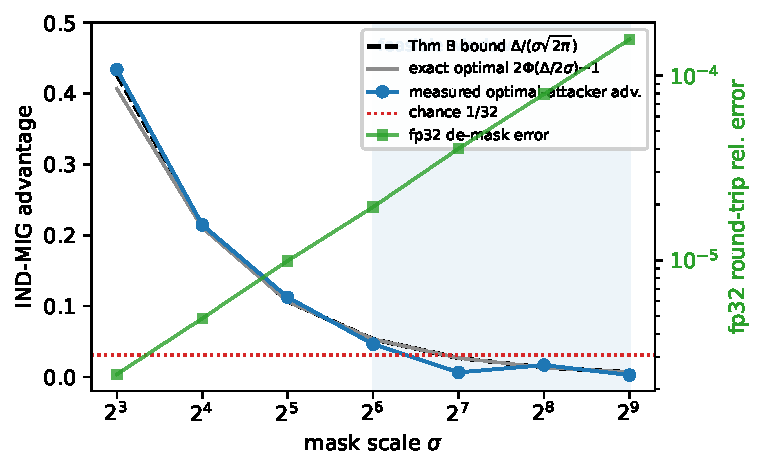
\includegraphics[width=\columnwidth]{figs/confidentiality_sweep.pdf}
\caption{RQ11. The measured optimal-attacker \textsc{IND-MIG} advantage (blue) tracks the Gaussian-mechanism bound of Theorem~\ref{thm:confidentiality} (dashed) and decays to the $1/32$ chance level, while the fp32 de-mask error (green, right axis) grows with $\sigma$ (Theorem~\ref{thm:precision}); the shaded band is the feasible window. Orthogonal protection is the $\sigma{=}0$ endpoint with advantage $1.0$.}
\label{fig:sweep}
\end{figure}

\textbf{The migration attacker is reduced to blind guessing.} Table~\ref{tab:ge} reports guessing entropy (mean rank of the true secret among $N{=}32$; $1$ = fully recovered, $(N{+}1)/2{=}16.5$ = chance). Orthogonal caches ($\sigma{=}0$) have guessing entropy $1.0$ on both models---the secret is always rank-1, i.e.\ zero residual uncertainty, consistent with Theorem~\ref{thm:impossible}. For any $\sigma\ge16$ the migration attacker's guessing entropy is at the chance level on both Qwen3-0.6B and Llama-3.2-1B: the affine mask leaves essentially the full $\log_2 N$ bits of uncertainty.

\begin{table}[t]
\centering
\caption{RQ11. Guessing entropy of the migration attacker (mean rank, $N{=}32$, chance $16.5$). Orthogonal ($\sigma{=}0$) fully recovers (GE $1.0$); affine leaves the secret at chance for $\sigma\ge16$.}
\label{tab:ge}
\begin{tabular}{@{}lcc@{}}
\toprule
$\sigma$ & Qwen3-0.6B & Llama-3.2-1B \\
\midrule
0 (orthogonal) & 1.0 & 1.0 \\
16 & 15.5 & 17.2 \\
64 & 15.6 & 17.4 \\
128 & 15.7 & 17.2 \\
512 & 15.8 & 17.2 \\
\bottomrule
\end{tabular}
\end{table}

\textbf{Adaptive attacks define the exact boundary.} Table~\ref{tab:adaptive} reports two attackers stronger than single-shot matching. Same-session known-plaintext recovers \emph{both} the basis (orthogonal Procrustes on cross-prompt differences, which cancel the mask) and the mask itself, stripping a held-out cache to residual $0.000$---so the affine mask, like the orthogonal basis, is broken under same-session KPA, and its protection is only for the migration attacker; under a refreshed nonce the recovered $(O,M)$ do not transfer (residual $\gg 1$). The averaging attacker, which needs the same secret cached many times under independent per-write masks, stays at chance through $10^5$ observations and reaches only top-1 $0.50$ (Qwen3) or chance (Llama) at $10^6$ observations: recovery requires $\Theta((\sigma\sqrt{d}/\lVert X\rVert)^2)$ identical re-cachings, an impractical capability. Together with the differencing attack (Table~\ref{tab:differencing}), these state the boundary precisely: the per-write nonce stops differencing, session refresh stops cross-session transfer, and same-session aligned known-plaintext is the designed non-goal.

\begin{table}[t]
\centering
\caption{RQ11. Adaptive attacks on the affine mask (std~128). KPA rows report strip residual (same-session $\to 0$ = broken; refreshed nonce $\gg 1$ = safe); averaging rows report top-1, needing $\ge 10^6$ identical re-cachings.}
\label{tab:adaptive}
\begin{tabular}{@{}lcc@{}}
\toprule
Attack & Qwen3-0.6B & Llama-3.2-1B \\
\midrule
KPA, same session & 0.000 & 0.000 \\
KPA, refreshed nonce & $\gg 1$ & $\gg 1$ \\
Averaging, $10^5$ obs. & 0.075 & 0.000 \\
Averaging, $10^6$ obs. & 0.500 & 0.025 \\
\bottomrule
\end{tabular}
\end{table}

\textbf{No plaintext is materialized, in use or at rest.} Finally, Table~\ref{tab:materialize} operationalizes Definition~\ref{def:inuse}. Encrypt-at-rest must decrypt a cache page to plaintext $V$ before attention, so an in-use memory snapshot yields plaintext and layer-0 V-inversion recovers every token (top-1 $1.000$, the RQ1 baseline). Orthogonal and affine \sys{} compute on the rotated coordinate $VO$ and never produce model-native plaintext anywhere in the memory hierarchy, so the same inversion on an in-use snapshot fails (top-1 $0.000$, the RQ2 cache-defense result). This is the property that distinguishes \sys{} from encryption even granting equal at-rest key handling.

\begin{table}[t]
\centering
\caption{RQ11. In-use materialization (Definition~\ref{def:inuse}). Layer-0 V-inversion top-1 on the tensor that attention actually consumes; only encrypt-at-rest exposes plaintext.}
\label{tab:materialize}
\begin{tabular}{@{}lcc@{}}
\toprule
Scheme & In-use tensor & V-inv \\
\midrule
AES-at-rest (decrypted) & plaintext $V$ & 1.000 \\
\sys{}, orth./affine & rotated $VO$ & \best{0.000} \\
\bottomrule
\end{tabular}
\end{table}

\textbf{Answer to RQ11:} The measured \textsc{IND-MIG} advantage tracks the Gaussian-mechanism bound of Theorem~\ref{thm:confidentiality} across $\sigma$ and decays to chance; the migration attacker's guessing entropy is at the $16.5$ chance level for $\sigma\ge16$ on both models (versus $1.0$ for orthogonal); same-session KPA is the precise non-goal while differencing, cross-session transfer, and averaging through $10^5$ observations are all defeated; and no plaintext K/V is materialized in use or at rest.

\subsection{Open Evaluation Gaps}

The Route~B experiments close the largest earlier gaps: the candidate audit now extends to $N=1000$ (RQ7) and confirms the advantage is flat in the candidate-set size, the differencing attack and its nonce fix are validated on real caches (RQ8), the head-to-head against encrypt-at-rest quantifies the materialization/throughput tradeoff (RQ9), and the PUF/FE assumptions are discharged in simulation (RQ10). Three gaps remain before submission. First, although the real-context PII benchmark covers public CC-News articles and real Enron emails, the secrets themselves are still seeded synthetically with exact scoring rather than mined from genuinely private records. Second, the PUF is simulated; RQ10 discharges the assumptions in software, but real FPGA traces are still needed to validate physical min-entropy, reliability, and helper-data leakage. Third, performance uses the unoptimized PyTorch wrapper: the orthogonal path composes with fused \texttt{scaled\_dot\_product\_attention} (Section~\ref{sec:discussion}), but fp16 FlashAttention and a fused affine de-masking cache-load kernel remain future work.
